\documentclass[11pt,twocolumn]{article}

\usepackage[utf8]{inputenc}
\usepackage[T1]{fontenc}
\usepackage{lmodern}
\usepackage[margin=0.75in]{geometry}
\usepackage{microtype}
\usepackage{amsmath,amssymb}
\usepackage{booktabs}
\usepackage{graphicx}
\usepackage{hyperref}
\usepackage{natbib}
\usepackage{caption}
\usepackage{array}
\usepackage{makecell}
\usepackage{xcolor}
\usepackage{enumitem}
\usepackage{seqsplit}
\usepackage{xurl}

\hypersetup{
  colorlinks=true,
  linkcolor=blue!50!black,
  citecolor=blue!50!black,
  urlcolor=blue!50!black,
  breaklinks=true
}

\setlength{\columnsep}{0.25in}
\setlength{\emergencystretch}{4em}

\begin{document}
\sloppy

\twocolumn[{
\begin{center}
{\LARGE\bfseries The Dark Triad as a Multi-Layered Structure: A Triangulation of Classical Psychometrics and Explainable Machine Learning for Testing the Distinctiveness and Convergence of Machiavellianism, Psychopathy, and Narcissism\par}
\vspace{1.2em}

{\large\bfseries Sabihe Khorshidi\par}
\vspace{0.2em}
{\small Independent Researcher, Tehran, Iran\par}
{\small Psychology Specialist, Project Lead\par}
{\small ORCID: \href{https://orcid.org/0009-0002-1060-4214}{\texttt{0009-0002-1060-4214}}\par}
{\small\texttt{sabihekhorshidy@gmail.com}\par}
\vspace{0.9em}

{\large\bfseries Kian Mansouri Jamshidi\par}
\vspace{0.2em}
{\small Independent Researcher, Tehran, Iran\par}
{\small Lead, Explainable AI (XAI)\par}
{\small ORCID: \href{https://orcid.org/0009-0001-3817-2305}{\texttt{0009-0001-3817-2305}}\par}
{\small\texttt{sirkianmj@gmail.com}\par}
\end{center}
\vspace{0.5em}
}]

\noindent\rule{\linewidth}{0.4pt}
\noindent\textbf{Abstract.} Since its introduction, the Dark Triad---Machiavellianism, psychopathy, and narcissism---has raised the question of whether these traits are distinct or manifestations of a shared Dark Core. Prior work relied on linear CFA/OLS, which cannot detect nonlinearities. Using existing Dirty Dozen data from community ($N = 5{,}902$), student ($N = 2{,}071$), and representative ($N = 1{,}492$) samples, we applied the Dark Triad Triangulation (DT$^3$) framework across five layers: network psychometrics, supervised machine learning, counterfactual tipping points, semantic embeddings, and robustness testing. A bifactor CFA ($\chi^2(42) = 1109.75$, CFI = .965, TLI = .944, RMSEA = .066) outperformed the correlated three-factor model (CFI = .941, RMSEA = .077); ECV = .576, $\omega_H = .734$, and subscale $\omega_{HS} = .036/.450/.532$ (Machiavellianism/Psychopathy/Narcissism), indicating substantial specific variance for the latter two only; latent factor correlations were $r = .62$ (Machiavellianism--Psychopathy), $.61$ (Machiavellianism--Narcissism), and $.36$ (Psychopathy--Narcissism). The 12-item network yielded three communities, but in the full 88-item space all Dark Triad items merged into one Dark Core. Supervised predictors diverged (agreeableness, empathy, and age, respectively), CKA indicated representational distinctiveness, and semantic clustering partially separated traits (ARI = .505, $p = .007$). Linear models matched XGBoost, indicating that the explainable-ML contribution is interpretive rather than predictive. Out-of-sample $R^2$ (.13--.22) limits inferences. Findings support a strong general Dark factor, with Psychopathy and Narcissism retaining specific variance but Machiavellianism not.
\noindent\rule{\linewidth}{0.4pt}

\par\vspace{0.5em}
\noindent\textbf{Keywords:} Dark Triad of personality; Dark Core of Personality; explainable machine learning; SHAP; network psychometrics; Machiavellianism; psychopathy; narcissism; out-of-sample validation

\section{Introduction}

Since \citet{paulhus2002} first grouped together the three subclinical traits of Machiavellianism, psychopathy, and narcissism under the label ``Dark Triad,'' this framework has become one of the most widely used research constructs in personality, organizational, and social psychology. Much of its appeal derives from a foundational hypothesis: although the three traits correlate with one another, each represents a relatively distinct behavioral, motivational, and interpersonal pattern. Brief instruments such as the 12-item Dirty Dozen (DTDD; \citealp{jonason2010}) and the Short Dark Triad (SD3; \citealp{jones2014}) enabled this research to be conducted at scale in non-clinical populations.

Meta-analytic work has repeatedly questioned the distinctiveness of these traits, with evidence of substantial redundancy between the Dark Triad and the Five-Factor Model \citep{oboyle2015}, pronounced overlap between Machiavellianism and psychopathy \citep{muris2017}, and heterogeneous empathy profiles across the three traits \citep{shukla2025}. The DTDD's factor structure has been the subject of recent meta-analytic SEM investigation \citep{knitter2025}, and machine-learning prediction of Dark Triad traits has gained considerable traction \citep{leberecht2026}.

From the outset, a serious controversy emerged regarding the true independence of these traits. A meta-analysis by \citet{vize2018} showed that although the nomological networks of the three traits differ, these differences are often small and situated at the margins of a larger shared core; the Machiavellianism--psychopathy overlap in particular is so pronounced that \citet{miller2017} explicitly asked whether it constitutes ``a distinction without a difference.'' In response, \citet{moshagen2018} proposed the ``Dark Factor of Personality'' (D): a basic tendency to maximize one's own utility at others' expense, accompanied by corresponding justifying beliefs. From this perspective, Machiavellianism, psychopathy, narcissism, and related dark traits are surface manifestations of a single underlying disposition rather than fully independent constructs.

Empirical work on this controversy has relied almost entirely on classical linear methods---CFA and OLS regression. These methods have two important limitations. First, both assume linear, additive relationships and are thus ill-suited to detecting thresholds, higher-order interactions, or nonlinear functional forms. Second, latent factor correlations---typically used to adjudicate distinctiveness---are a summary, unidimensional index that cannot reveal whether the predictive pattern, internal representation, or semantic structure of a trait is genuinely distinct from that of its neighbors.

This motivates a testable middle-ground hypothesis: Machiavellianism, psychopathy, and narcissism share a meaningful common component (consistent with Dark Core theory; \citealp{moshagen2018}) while retaining distinctive patterns across psychometric structure, relational networks, predictive drivers, feature importance, and computational representations.

\subsection{Aims and Research Questions}

This study addresses three questions:
\begin{enumerate}[leftmargin=1.2em,itemsep=0pt,topsep=2pt]
\item When examined with supervised and unsupervised methods beyond linear factor analysis, do the three traits exhibit distinctive predictive patterns, internal representations, and semantic structures?
\item How does this distinctiveness change when the variable space expands from the 12 DTDD items to the full personality space (Big Five, empathy)?
\item Which trait, if any, shows the greatest functional overlap with another, and with which personality constructs is this overlap associated?
\end{enumerate}

The primary innovation is the integration of five independent computational layers within a single, reproducible DT$^3$ framework, enabling direct comparison across methods without sample or tool confounds.

\section{Methods}

\subsection{Participants and Samples}

Data were drawn from the Czech validation study of the DTDD \citep{zivna2025}, with the underlying project materials and de-identified data available at the associated OSF repository \citep{zivna2023osf}. Raw files were reprocessed to ensure feature alignment across analysis layers; reported sample sizes may therefore differ slightly from the original validation study due to inclusion/exclusion criteria. Unless otherwise stated, all psychometric indices reported in the present article (including the CFA fit statistics in Table~\ref{tab:cfa} and the reliability estimates in Table~\ref{tab:alpha}) were re-estimated on the present analytic subsamples rather than copied from the original validation study; small numerical differences from the published values are therefore expected.

The full OSF release contains 17,517 raw records; preprocessing (Section~2.3) retained 9,465 usable cases, distributed across three samples: a community sample ($N = 5{,}902$), a student sample ($N = 2{,}071$), and a national representative sample ($N = 1{,}492$). Case-wise exclusion for missing auxiliary data (particularly the Rosenberg Self-Esteem Scale, RSES, essentially absent in the representative sample; exclusion threshold $>90\%$ missing) reduced analytic $N$s per analysis (e.g., Layer~5 cross-validation for the community sample: $N = 5{,}215$). An independent subsample of 61 matched participants (from 3,913 test--retest records) was used for ICC estimation.

The community sample served as the training set and the representative sample as a fully held-out test set for all supervised components (Layers~2, 3, 5); the representative sample was untouched during fitting, hyperparameter search, or feature selection, and used only once for final scoring. The student sample lacked auxiliary variables (Big Five, empathy, demographics) required for feature alignment and was excluded from predictive-modeling layers, retained only for analyses not requiring the full auxiliary set (e.g., reliability).

\subsection{Instruments}

The Dark Triad was measured with the Dirty Dozen \citep{jonason2010}, 12 items on a 7-point Likert scale, four items per trait: Machiavellianism (manipulativeness, deceitfulness, flattery, instrumental exploitation), psychopathy (lack of remorse, moral indifference, callousness, cynicism), and narcissism (need for admiration, attention-seeking, status-seeking, entitlement). The Big Five was assessed with the BFI, empathy with the Toronto Empathy Questionnaire (TEQ), and self-esteem with the RSES. The RSES was available in the community and student samples and was included in the baseline OLS; it was excluded from Layers~2--5 because it was essentially absent from the representative sample.

\subsection{Data Preprocessing}

Steps included: (a) restricting age to 18--100 years; (b) removing flagged ``speeders''/low-quality responders; (c) using a minimum item count for composite scores rather than zero-imputation; and (d) requiring $\approx 80\%$ minimum item completion for BFI/TEQ/RSES composites.

\subsection{Baseline Psychometrics}

All confirmatory factor analyses reported in Table~\ref{tab:cfa} were estimated with \texttt{semopy} (Python 3.11). Internal consistency was estimated with Cronbach's $\alpha$ and McDonald's $\omega$. In the final pipeline, $\omega$ converged on the $\alpha$ estimate to within .02 in all nine subscale $\times$ sample cells (range: 0 to .017), consistent with the near-tau-equivalence of the four DTDD items per trait (see Section~\ref{sec:limitations}). Temporal stability used ICC(2,1) on the test--retest subsample; factor structure used CFA comparing one-, two-, and three-factor models, reporting $\chi^2$, df, CFI, TLI, and RMSEA. In addition to the three competing correlated-factor models (one-, two-, and three-factor), we estimated a bifactor model specifying one general Dark factor loading on all 12 items and three orthogonal specific factors (Machiavellianism, Psychopathy, Narcissism). Bifactor dimensionality indices---explained common variance (ECV), the reliability of the general factor ($\omega_H$), and the reliability of each specific factor given the general factor ($\omega_{HS,k}$, computed separately for Machiavellianism, Psychopathy, and Narcissism)---were computed following \citet{rodriguez2016}, with item uniqueness defined as $u_i^2 = 1 - \lambda_{Gi}^2 - \lambda_{Si}^2$ and total uniqueness entered in the denominator of $\omega_H$. Two theoretically motivated 2-factor specifications were also estimated: one merging Machiavellianism with Psychopathy (the \citealp{miller2017} redundancy hypothesis) and one merging Machiavellianism with Narcissism (the semantic-overlap hypothesis from Layer~4). Nomological networks were estimated via standardized OLS regression (predictors: Big Five, empathy, self-esteem). All CFAs were estimated on continuous Pearson correlations using \texttt{semopy}. SRMR was not included in the reported fit statistics; ordinal WLSMV estimation with polychoric correlations is a further recommended sensitivity check that was not run in the present analysis.

\subsection{Computational Methodology: The \texorpdfstring{DT$^3$}{DT3} Triangulation Framework}

\subsubsection{Out-of-Sample Evaluation Strategy}

All supervised components (Layers~2, 3, 5) were trained exclusively on the community sample and evaluated once on the held-out representative sample; architectures, hyperparameters, and preprocessing were finalized via internal cross-validation within the community sample only. Network analyses (Layer~1) were conducted in Python 3.11 using \texttt{networkx} and \texttt{scikit-learn}'s \texttt{GraphicalLasso}, with an EBIC-style L1-penalty grid search (a Python reimplementation of the procedure described by \citealp{epskamp2018}); Louvain community detection used \texttt{python-louvain}. Supervised and semantic layers were implemented in Python (\texttt{xgboost}, \texttt{shap}, \texttt{scikit-learn}, \texttt{\seqsplit{sentence-transformers}}, \texttt{gplearn}).

\subsubsection{Layer 1: Unsupervised Structural Networks}

Structural relationships were modeled via Graphical LASSO regularized with EBIC (\texttt{EBICglasso}; \citealp{epskamp2018}), with Louvain community detection \citep{blondel2008}. Two specifications were estimated: a DTDD-only network (the 12 core DTDD items) and a full-item network of 88 nodes comprising 44 BFI items, 15 DTDD items (the 12 core items plus three Czech-variant items DTDD\_1g, DTDD\_1i, and DTDD\_1ma), 10 RSES items, and 19 TEQ items (the 16 core items plus three reverse-scored variants TEQ\_CON\_2, TEQ\_CON\_4, and TEQ\_CON\_14). Because the 10 RSES items were absent from the representative sample, this network was estimated on the pooled dataset with pairwise-deletion correlations rather than complete cases (see Section~3.2).

\subsubsection{Layer 2: Supervised Divergence and Representational Similarity}

Trait scores were modeled with Gradient-Boosted Decision Trees (XGBoost; \citealp{chen2016}), chosen for detecting nonlinear thresholds and interactions without OLS assumptions. Separate regressors per trait used an identical predictor set (age, Big Five, TEQ). A Shared-Trunk Multi-Task Neural Network (input $\rightarrow$ 128-d projection $\rightarrow$ two residual blocks $\rightarrow$ dropout $\rightarrow$ three output heads; Adam, lr $= 0.001$, weight decay $1\times10^{-4}$, batch size 128, 300 epochs, ReduceLROnPlateau) was trained in parallel. Representational geometry across trait-specific pathways was compared via Centered Kernel Alignment (CKA; \citealp{kornblith2019}), benchmarked against a label-permutation null (network retrained per permutation). Symbolic regression via evolutionary search (\texttt{gplearn}) additionally identified trait-specific functional forms without a priori shape constraints. As a cross-architecture reference, Random Forest and Elastic-Net regressors were also trained on the identical split (Rashomon Set analysis; see Layer~5).

\subsubsection{Layer 3: Counterfactual Tipping-Point Analysis}

A deterministic grid-search perturbation method \citep{wachter2017} quantified the minimal single-feature change required to shift an above-median case below the median, holding all other features constant. Age was held immutable and excluded from the search space. The outcome metric was the percentage of above-median cases for which perturbing the primary feature sufficed to cross below the median.

\subsubsection{Layer 4: Semantic Embeddings}

The original English DTDD item texts from \citet{jonason2010}---not the Czech translations administered to participants---were encoded with all-MiniLM-L6-v2 (SentenceTransformer family; \citealp{reimers2019}), followed by hierarchical agglomerative clustering (cosine distance, average linkage; $k = 3$ fixed a priori). Cluster assignments were compared to a priori trait labels via the Adjusted Rand Index (ARI), benchmarked against a 1,000-permutation null.

\subsubsection{Layer 5: Feature Importance and Robustness Testing}

Local/global feature importance used SHAP (TreeExplainer; \citealp{lundberg2017}). A SHAP Divergence Index (SDI)---a project-specific metric, mean pairwise cosine distance among mean absolute SHAP vectors---was benchmarked against a null built from 500 refits on randomly shuffled/recombined ``pseudo-traits'' derived from the same 12 items (limitation: not fully independent of the measurement system; Section~\ref{sec:limitations}). Individual heterogeneity was assessed via Gaussian Mixture Models on local SHAP vectors (BIC-selected components). Architecture robustness was assessed via a Rashomon Set analysis \citep{fisher2019} comparing out-of-sample $R^2$ across XGBoost, Random Forest, and Elastic-Net on an identical split.

\subsection{Ethical Considerations, Reproducibility, and Data/Code Availability}

This study is a secondary analysis of existing, de-identified data from the Czech validation study of the Dark Triad Dirty Dozen. The original human-subject research was conducted by the Olomouc University Social Health Institute (OUSH), Palacky University in Olomouc, Czech Republic. Adult participants provided informed consent, and the original study received ethical approval from the Ethics Committee of the Faculty of Theology of Palacky University in Olomouc (Approval No.\ 2020/4). The present authors were not involved in participant recruitment or the original data collection and did not conduct any new human-subject research.

Complete preprocessing and analysis code, validation materials, execution logs, and results tables are maintained in a public repository (\url{https://github.com/sirkianmj/dark_triad_triangulation}), with software versions documented through environment files (e.g., \texttt{environment\_dt3.yml} for the Python 3.11 pipeline). As the present analysis is exploratory and non-preregistered, the findings are hypothesis-generating.

\section{Results}

\subsection{Baseline Psychometrics}
\label{sec:baseline}

All baseline indices below were re-estimated on the present analytic subsamples (see Section~2.1); they therefore differ slightly from those reported in the original validation study \citep{zivna2025}. Internal consistency was acceptable for Machiavellianism ($\alpha = .802$--$.840$) and narcissism ($\alpha = .811$--$.846$) across all three samples, and marginal for psychopathy ($\alpha = .621$--$.763$), reaching its lowest value in the student sample ($\alpha = .621$, $\omega = .638$; Table~\ref{tab:alpha}). Temporal stability over the 61-pair retest subsample replicated this ordering: ICC(2,1) $= .826$, 95\% CI $[.726, .892]$ for Machiavellianism; $.836$ $[.741, .899]$ for narcissism; and $.637$ $[.464, .767]$ for psychopathy, all $p < .001$. The convergence of lower $\alpha$ and lower ICC for psychopathy is discussed in Section~\ref{sec:limitations} as a psychometric limitation of the DTDD psychopathy subscale.

\begin{table*}[ht]
\centering
\caption{Internal consistency ($\alpha$ / $\omega$) by trait and sample (re-estimated on the present analytic subsamples).}
\label{tab:alpha}
\small
\begin{tabular}{lcccc}
\toprule
Sample & $N$ & Machiavellianism $\alpha$ / $\omega$ & Psychopathy $\alpha$ / $\omega$ & Narcissism $\alpha$ / $\omega$ \\
\midrule
Community      & 5{,}902 & .828 / .828 & .763 / .771 & .846 / .850 \\
Student        & 2{,}071 & .802 / .804 & \textbf{.621 / .638} & .833 / .837 \\
Representative & 1{,}492 & .840 / .840 & .710 / .717 & .811 / .817 \\
\bottomrule
\end{tabular}
\end{table*}

The three-factor correlated model ($\chi^2 = 1838.65$, $df = 51$, CFI = .941, TLI = .923, RMSEA = .077) outperformed both 2-factor specifications: merging Machiavellianism with Psychopathy yielded $\chi^2 = 4589.6$, $df = 53$, CFI = .849, TLI = .812, RMSEA = .120; merging Machiavellianism with Narcissism yielded $\chi^2 = 6278.64$, $df = 53$, CFI = .793, TLI = .743, RMSEA = .141. Both merges fit substantially worse than the free three-factor model, and the Machiavellianism--Narcissism merge fits \textit{worse} than the Machiavellianism--Psychopathy merge despite the two trait pairs having nearly identical latent correlations ($r = .606$ vs.\ $.623$). This dissociation indicates that a latent correlation between two traits does not predict how much collapsing them into a single factor costs in model fit---a caution against using $r$ as the sole index of trait distinctiveness (Figure~\ref{fig:cfa_comparison}). A bifactor model with one general Dark factor and three orthogonal specific factors fit better than the correlated three-factor model on every fit index ($\chi^2(42) = 1109.75$, CFI = .965, TLI = .944, RMSEA = .066; Table~\ref{tab:cfa}, Table~\ref{tab:bifactor_loadings}). Computation of the \citet{rodriguez2016} indices from the standardized loadings gives ECV = .576 and $\omega_H = .734$ for the general factor. The three specific factors diverge sharply: $\omega_{HS,M} = .036$, $\omega_{HS,P} = .450$, and $\omega_{HS,N} = .532$. Following the \citet{rodriguez2016} criterion that $\omega_{HS} < .50$ indicates a subscale whose unit-weighted composite is dominated by general-factor and error variance, this pattern indicates that the Machiavellianism specific factor retains virtually no reliable variance ($\omega_{HS,M} = .036$), Psychopathy falls below the .50 threshold ($\omega_{HS,P} = .450$), and only Narcissism marginally clears it ($\omega_{HS,N} = .532$). Item-level ECV was .988 for DTDD\_4m and .990 for DTDD\_1m, confirming that the Machiavellianism items are nearly pure indicators of $D$. Mean \textit{signed} specific loadings were $.154$ (M$_s$), $.516$ (P$_s$), and $.603$ (N$_s$); mean \textit{absolute} specific loadings were $.202$, $.516$, and $.603$, respectively. Machiavellianism is therefore best characterized as a near-pure indicator of the general Dark factor rather than as a specific dimension with substantial unique variance---a structural result that converges with its bridging position in the latent correlation matrix ($r = .623$ with Psychopathy, $r = .606$ with Narcissism) and with its intermediate role in Layers~1--5. Fit indices in the present analysis are from raw ML estimation; robust MLR estimation, as used by the original validation study \citep{zivna2025}, would inflate $\chi^2$ under non-normality.

\begin{table*}[ht]
\centering
\caption{Comparison of fit across five CFA specifications: 1-factor, 2-factor (two alternative merges), 3-factor correlated, and bifactor (community sample, $N = 5{,}902$; re-estimated in the present analysis).}
\label{tab:cfa}
\footnotesize
\begin{tabular}{lcccccc}
\toprule
Model & $\chi^2$ & $df$ & $\chi^2/df$ & CFI & TLI & RMSEA \\
\midrule
1-factor & 9505.75 & 54 & 176.03 & .686 & .616 & .172 \\
2-factor (Mach.\ + Psych.\ merged) & 4589.60 & 53 & 86.60 & .849 & .812 & .120 \\
2-factor (Mach.\ + Narc.\ merged) & 6278.64 & 53 & 118.46 & .793 & .743 & .141 \\
3-factor (correlated) & 1838.65 & 51 & 36.05 & .941 & .923 & .077 \\
Bifactor (D + M$_s$ + P$_s$ + N$_s$) & 1109.75 & 42 & 26.42 & \textbf{.965} & \textbf{.944} & \textbf{.066} \\
\bottomrule
\end{tabular}
\par\smallskip
\footnotesize\raggedright
\textit{Note.} Mach.\ = Machiavellianism; Psych.\ = Psychopathy; Narc.\ = Narcissism; D = general Dark factor. Bifactor indices: ECV = .576; $\omega_H$ = .734; subscale $\omega_{HS}$ = .036 (Machiavellianism), .450 (Psychopathy), .532 (Narcissism). All models estimated with \texttt{semopy} (Python 3.11); SRMR not reported.
\end{table*}

\begin{figure*}[ht]
\centering
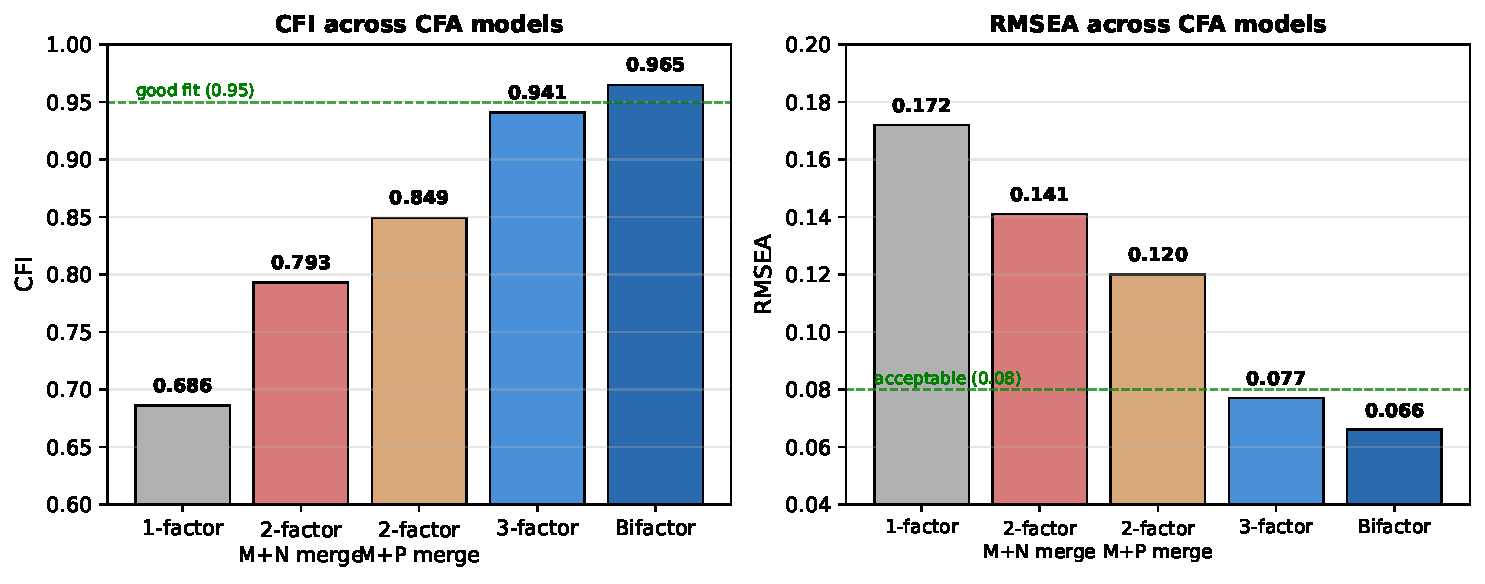
\includegraphics[width=\linewidth]{results/figures/baseline_cfa_comparison.pdf}
\caption{Comparative CFA fit across five specifications (community sample, $N = 5{,}902$). Both 2-factor merges fall below the free three-factor model on both CFI and RMSEA, and the Machiavellianism--Narcissism merge (CFI = .793, RMSEA = .141) fits worse than the Machiavellianism--Psychopathy merge (CFI = .849, RMSEA = .120) despite the two trait pairs having nearly identical latent correlations ($r = .606$ vs.\ $.623$). This dissociation between the magnitude of latent correlation and the merge penalty is the CFA counterpart to the semantic and feature-importance dissociation reported in Layers~3--4.}
\label{fig:cfa_comparison}
\end{figure*}

\begin{table}[ht]
\centering
\caption{Standardized bifactor loadings for the 12 DTDD items (community sample).}
\label{tab:bifactor_loadings}
\footnotesize
\begin{tabular}{lccc}
\toprule
Item & $D$ loading & Specific loading & Specific factor \\
\midrule
DTDD\_1m & .765 & .075 & M$_s$ \\
DTDD\_2m & .690 & .404 & M$_s$ \\
DTDD\_3m & .613 & .234 & M$_s$ \\
DTDD\_4m & .872 & $-.096$ & M$_s$ \\
\midrule
DTDD\_1p & .338 & .540 & P$_s$ \\
DTDD\_2p & .454 & .523 & P$_s$ \\
DTDD\_3p & .504 & .658 & P$_s$ \\
DTDD\_4p & .474 & .343 & P$_s$ \\
\midrule
DTDD\_1n & .478 & .710 & N$_s$ \\
DTDD\_2n & .407 & .685 & N$_s$ \\
DTDD\_3n & .452 & .601 & N$_s$ \\
DTDD\_4n & .534 & .415 & N$_s$ \\
\bottomrule
\end{tabular}
\par\smallskip
\footnotesize\raggedright
\textit{Note.} Subscale-specific hierarchical omega ($\omega_{HS}$) is .036 for Machiavellianism, .450 for Psychopathy, and .532 for Narcissism. Mean \textit{signed} specific loadings are $.154$, $.516$, and $.603$; mean \textit{absolute} specific loadings are $.202$, $.516$, and $.603$. One Machiavellianism item (DTDD\_4m) has a small negative loading on M$_s$ ($-.096$) while loading $.872$ on $D$, and item-level ECV for this item is $.988$.
\end{table}

\begin{table}[ht]
\centering
\caption{Latent factor correlations in the three-factor model (community sample).}
\label{tab:latentcor}
\footnotesize
\begin{tabular}{lccc}
\toprule
 & Mach. & Psych. & Narc. \\
\midrule
Machiavellianism & ---   & .623 & .606 \\
Psychopathy      &       & ---  & \textbf{.363} \\
Narcissism       &       &      & ---  \\
\bottomrule
\end{tabular}
\end{table}

Machiavellianism shows relatively high correlations with both other traits, while psychopathy and narcissism show the least latent overlap---a bridging pattern for Machiavellianism that recurs in the computational layers (particularly Layers~1 and~4).

\begin{table*}[ht]
\centering
\caption{Standardized OLS regression summary (community sample; predictors: Big Five, empathy, self-esteem).}
\label{tab:ols}
\small
\begin{tabular}{lccc}
\toprule
Predictor & Machiavellianism $\beta$ & Psychopathy $\beta$ & Narcissism $\beta$ \\
\midrule
Agreeableness        & $-.328$\textsuperscript{***} & $-.306$\textsuperscript{***} & $-.198$\textsuperscript{***} \\
Conscientiousness    & $-.130$\textsuperscript{***} & $-.109$\textsuperscript{***} & $-.092$\textsuperscript{***} \\
Neuroticism          & $.031$ (ns)                  & $-.138$\textsuperscript{***} & $.120$\textsuperscript{***}  \\
Openness             & $.110$\textsuperscript{***}  & $.089$\textsuperscript{***}  & $.144$\textsuperscript{***}  \\
Extraversion         & $.136$\textsuperscript{***}  & $.058$\textsuperscript{**}   & $.153$\textsuperscript{***}  \\
Empathy (TEQ)        & $-.139$\textsuperscript{***} & $-.281$\textsuperscript{***} & $-.048$\textsuperscript{*}   \\
Self-esteem (RSES)   & $.100$\textsuperscript{***}  & $-.065$\textsuperscript{***} & $.096$\textsuperscript{***}  \\
\midrule
Adjusted $R^2$       & $.188$        & $.278$        & $.106$        \\
\bottomrule
\end{tabular}
\end{table*}

Psychopathy showed the best predictability (adjusted $R^2 = .278$) and the strongest dependence on low empathy; narcissism, uniquely, showed a positive relationship with extraversion and the lowest explained variance (adjusted $R^2 = .106$). Low agreeableness was the dominant shared predictor across all three traits.

\subsection{Layer 1: Unsupervised Structural Networks}

The EBICglasso network on the 12 DTDD indicators produced three Louvain communities corresponding exactly to the three theoretical traits (Figure~\ref{fig:network12}), confirming the three-factor structure from an independent network-psychometric perspective. When re-estimated in the full 88-item space (following positive-definite projection, $\alpha = 0.0346$), all Dark Triad items merged into a single Louvain community---termed the ``Dark Core Collapse'' (Figure~\ref{fig:network88}). Two caveats qualify this result. First, the 88-item space includes 44 BFI items, 15 DTDD items (12 core plus DTDD\_1g, DTDD\_1i, and DTDD\_1ma), 10 RSES items, and 19 TEQ items (16 core plus TEQ\_CON\_2, TEQ\_CON\_4, and TEQ\_CON\_14), despite the RSES being excluded from Layers~2--5 for missingness. Because RSES was essentially absent in the representative sample, complete-case analysis was impossible ($N_{\text{complete}} = 0$); the model was therefore estimated on pairwise-deletion correlations, with effective $N \approx 6{,}734$ and $P = 88$. Second, Louvain community detection returned 20 communities in the full-item space: the DTDD items collapsed into one, but most TEQ items formed singleton communities and \texttt{BFI\_A\_9} clustered with Extraversion. The fragmentation of the non-DTDD scales indicates that the 88-item network is not a well-behaved representation of the broader personality space, and the Dark Core Collapse should be read as ``the 12 DTDD items are more tightly intercorrelated with each other than with anything else in the space,'' rather than as direct evidence of a latent general factor. The bifactor CFA (Section~\ref{sec:baseline}) provides the direct structural evidence; the 88-item network is corroborative, not primary. Prior network analyses of the Dark Triad alongside the Five-Factor Model \citep{papageorgiou2019, wehner2021} did not systematically contrast DTDD-only and full-personality spaces in a single framework, so direct comparison with those results is limited.

\begin{figure}[ht]
\centering
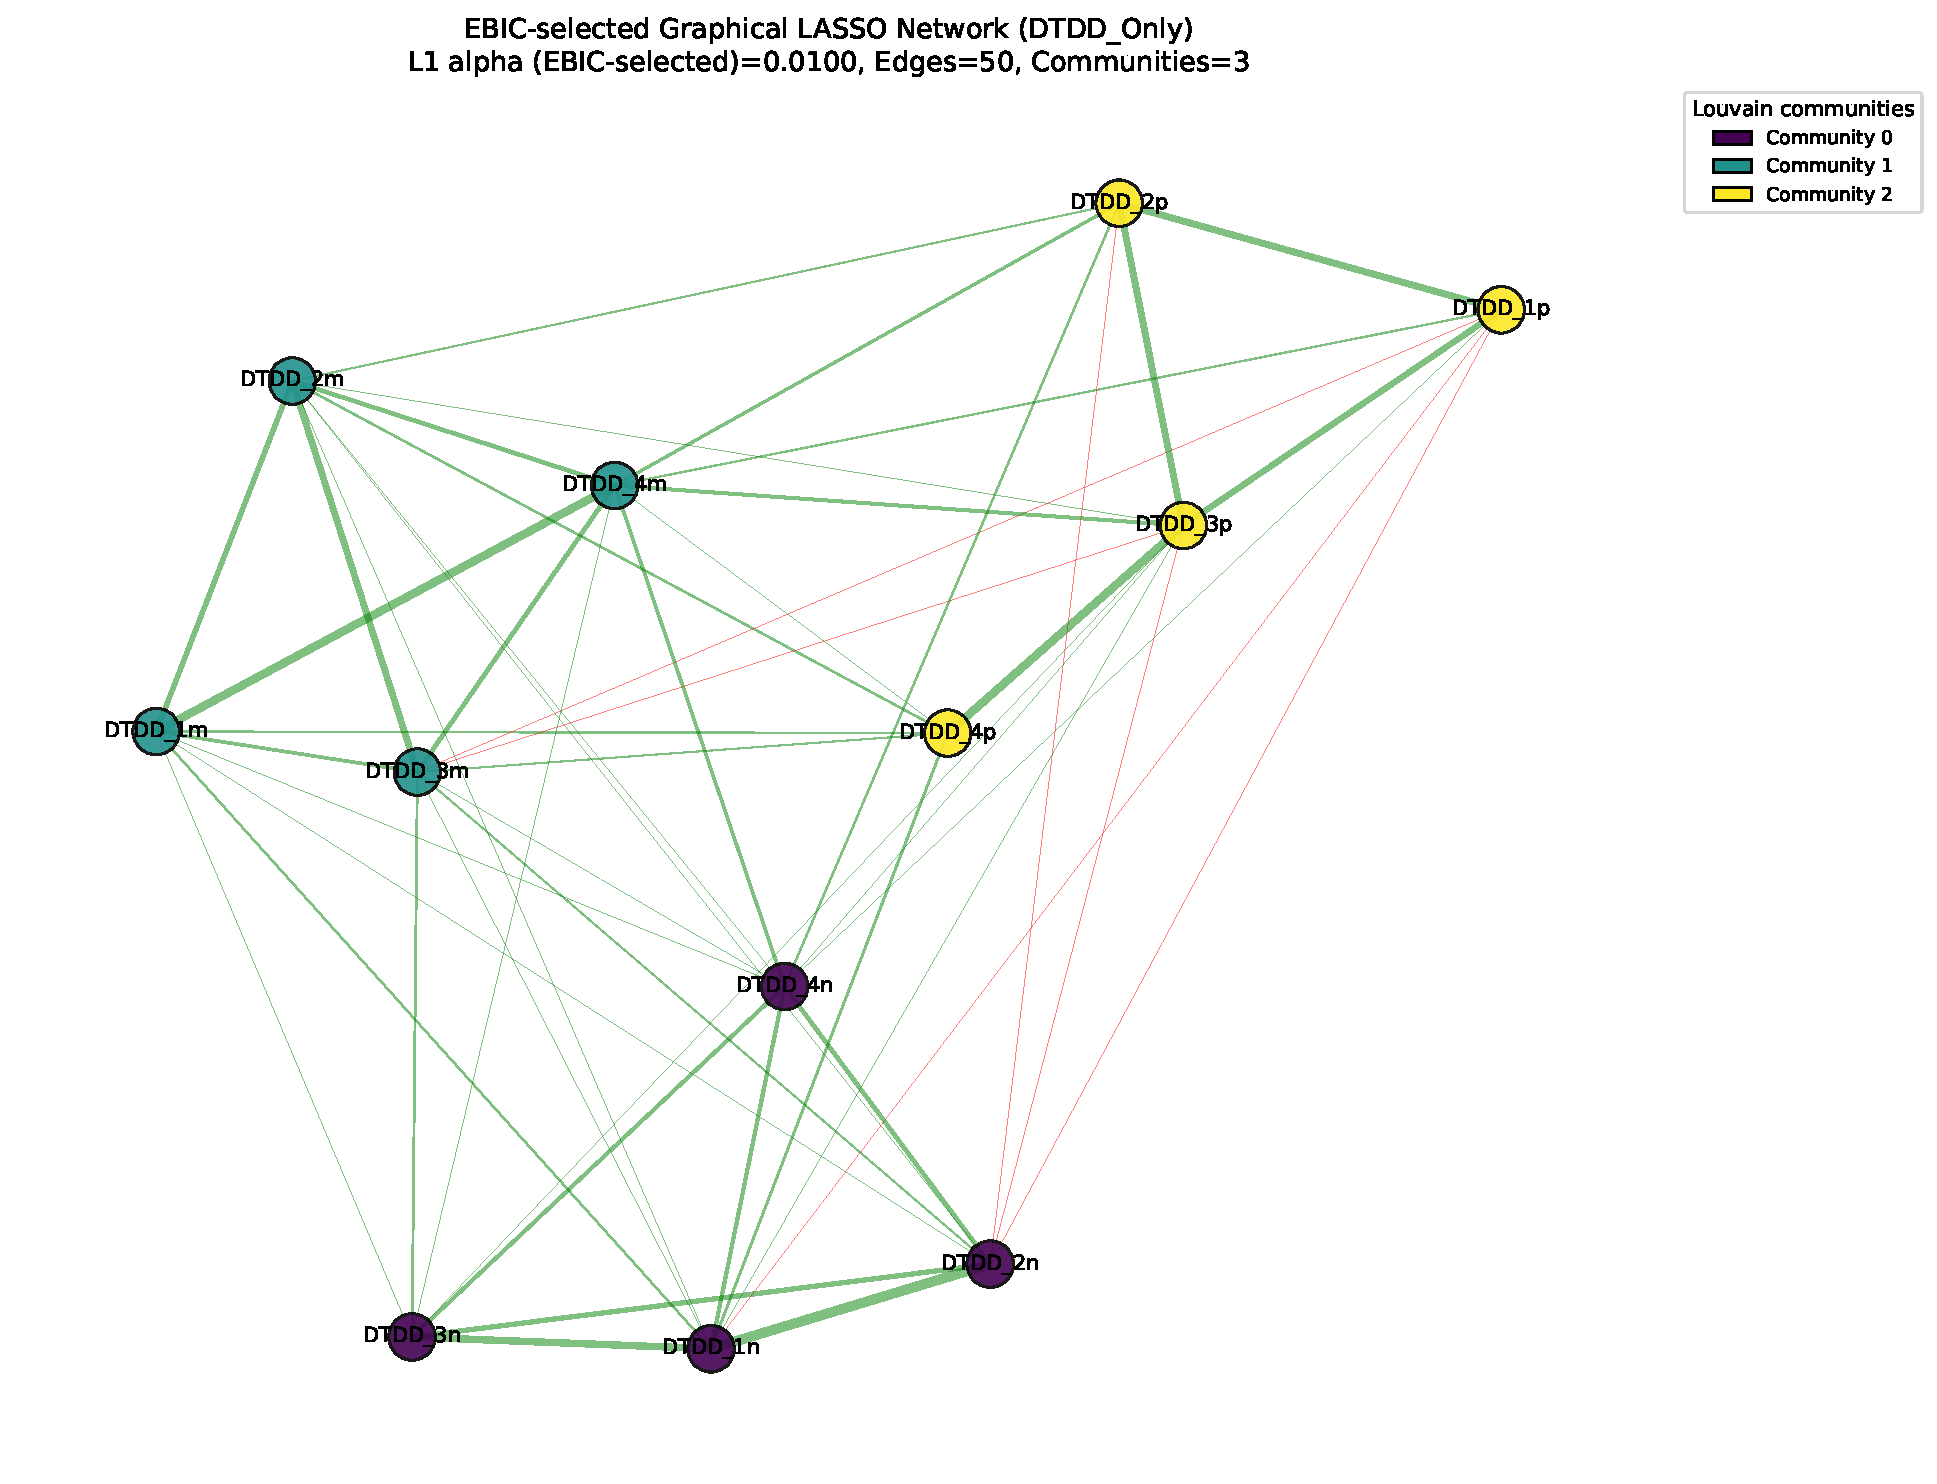
\includegraphics[width=\linewidth]{results/figures/layer1_ggm_network_DTDD_Only.pdf}
\caption{EBICglasso network on the 12 DTDD items, showing three Louvain communities corresponding to the three theoretical traits.}
\label{fig:network12}
\end{figure}

\begin{figure*}[ht]
\centering
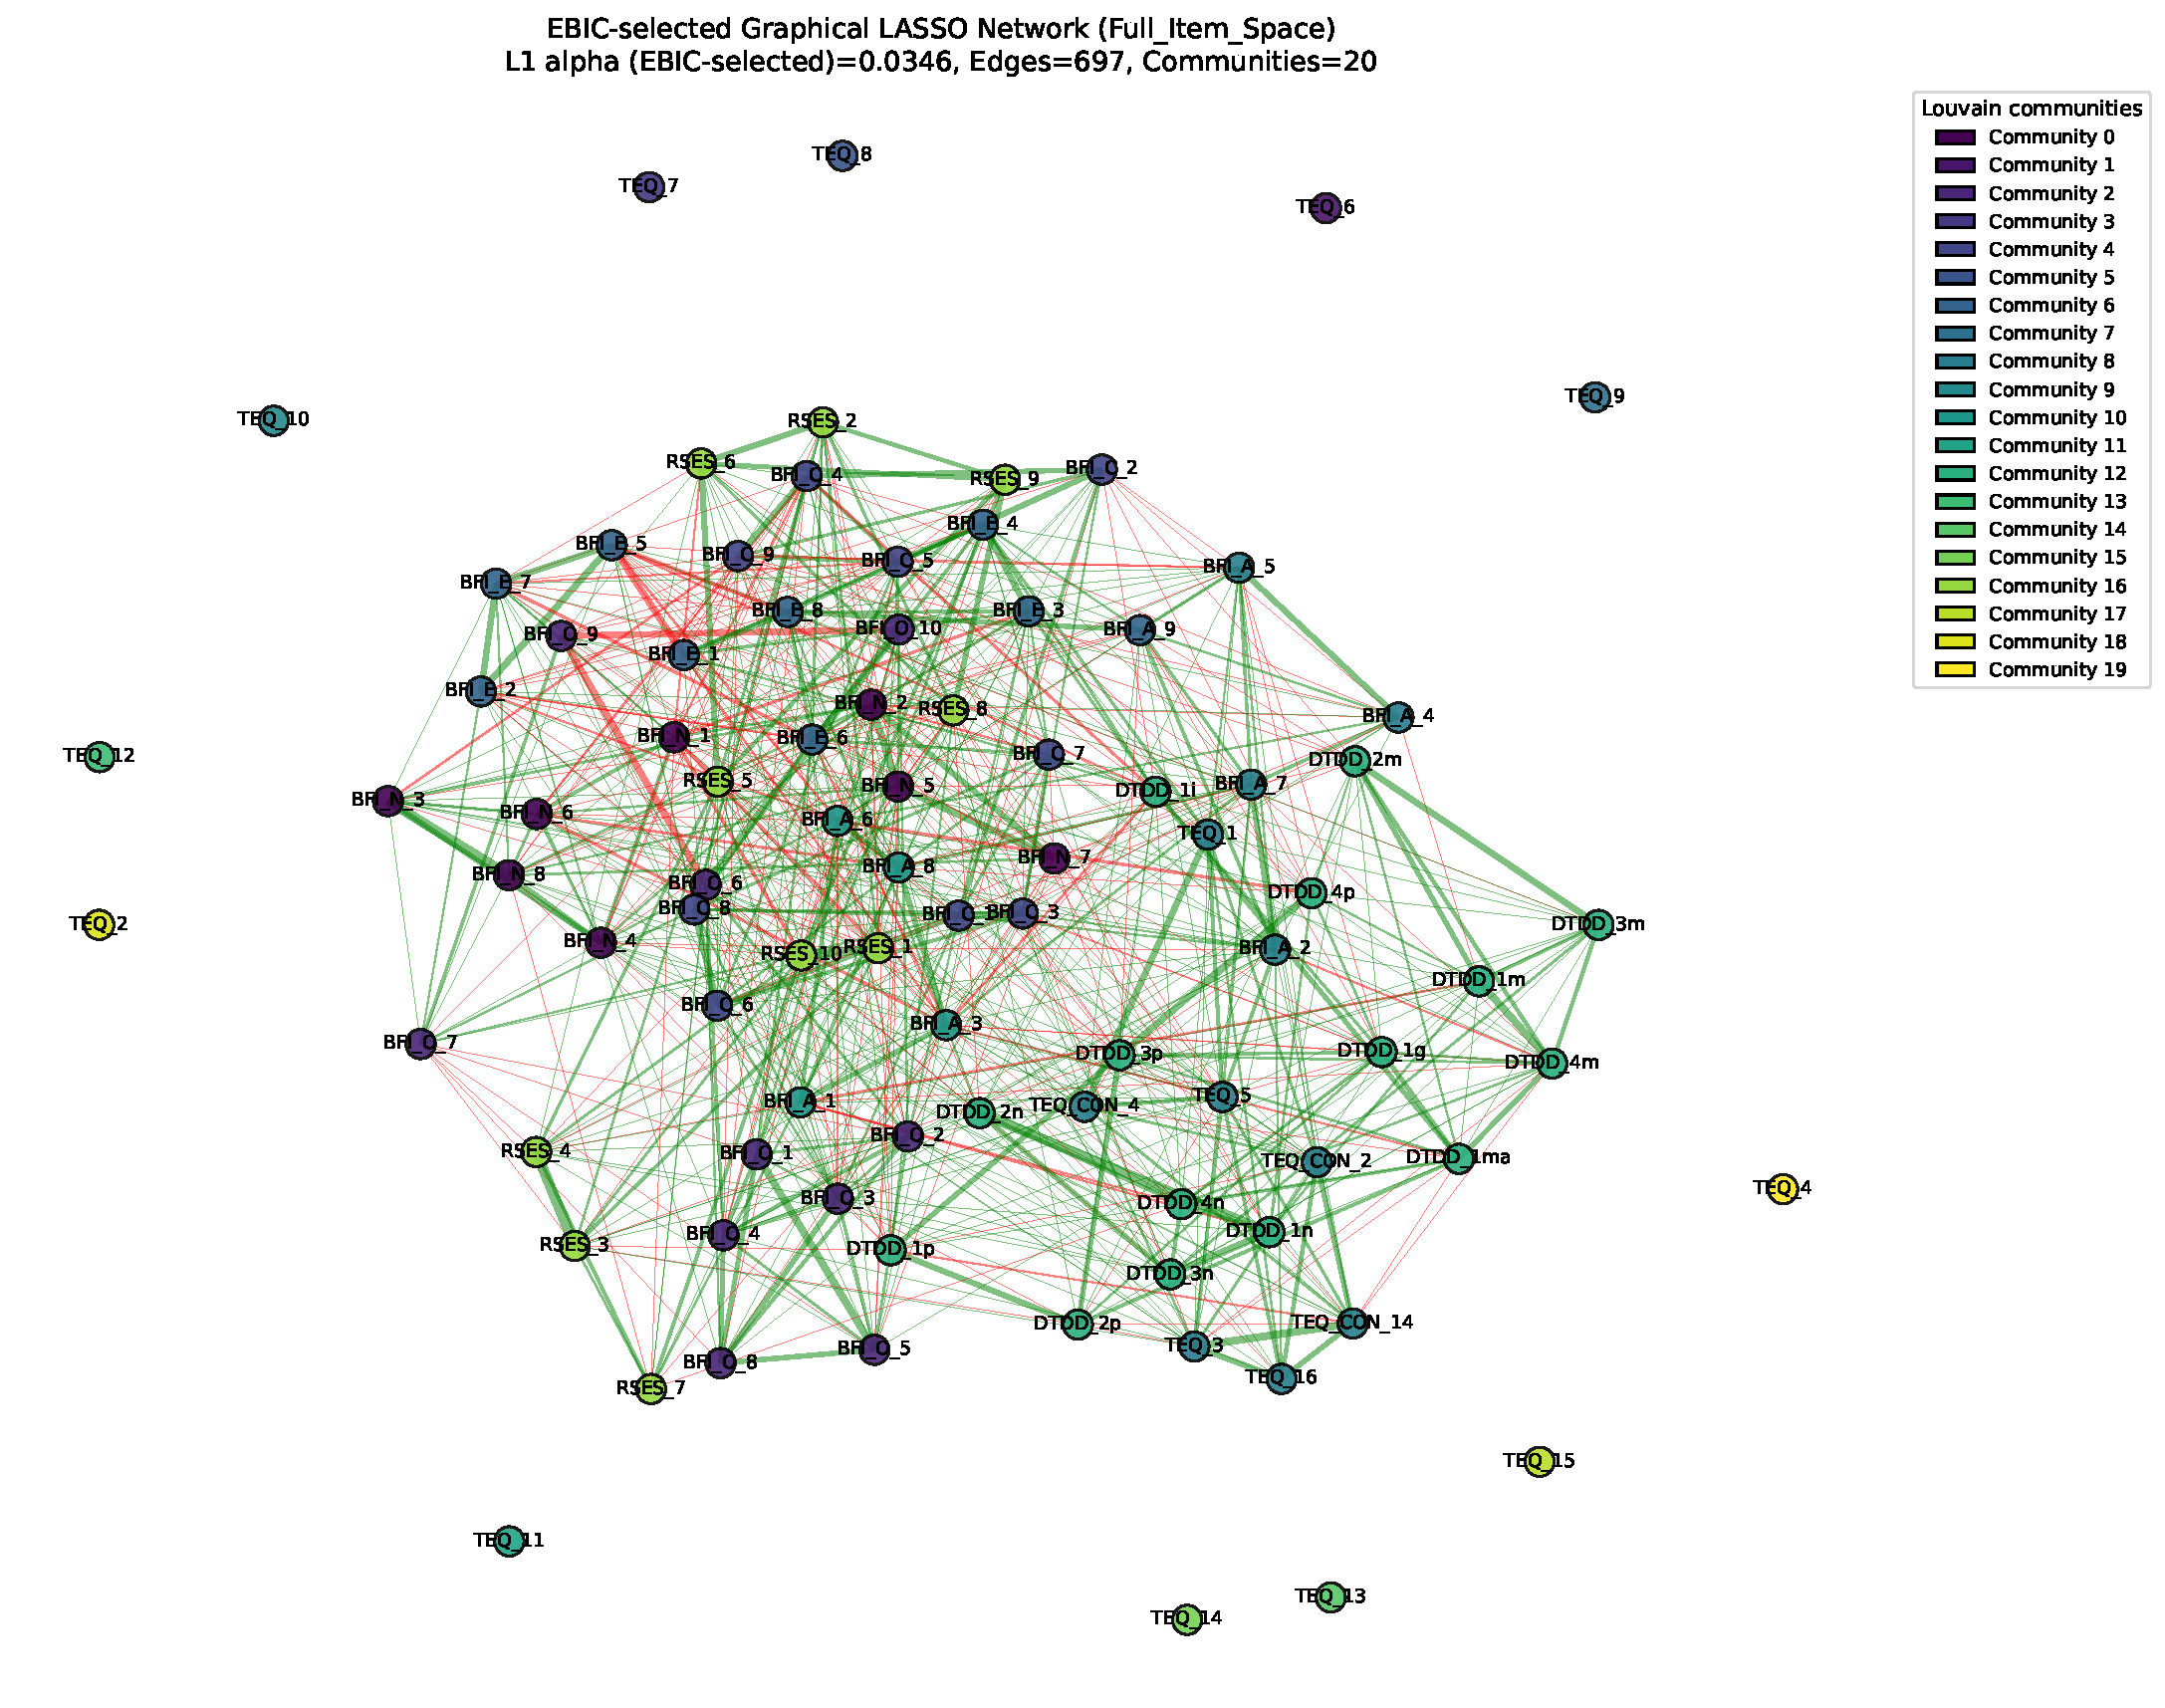
\includegraphics[width=0.85\linewidth]{results/figures/layer1_ggm_network_Full_Item_Space.pdf}
\caption{EBICglasso network in the full 88-item personality space. All twelve DTDD items merge into a single Louvain community (the ``Dark Core Collapse'').}
\label{fig:network88}
\end{figure*}

\subsection{Layer 2: Supervised Divergence and Representational Similarity}
\label{sec:layer2}

Out-of-sample $R^2$ ranged from .132 to .218 (Table~\ref{tab:xgb}), indicating that the supervised models explain only a limited portion of trait variance (Section~\ref{sec:limitations}). The traits shared low agreeableness as a dominant predictor but diverged in secondary structure: empathy was specific to psychopathy, extraversion and openness to narcissism, and age to narcissism in the supervised layers. SHAP interaction analysis found three distinct high-order interaction pairs across the three traits; the single strongest interaction overall belonged to psychopathy (agreeableness $\times$ empathy; strength $= .186$). Symbolic regression discovered three trait-specific functional forms (iteration $R^2$: Machiavellianism $= .093$, psychopathy $= .184$, narcissism $= .143$); given the complexity and overfitting risk of the recovered equations, these are treated as supplementary rather than primary evidence (Section~\ref{sec:limitations}). The multi-task network's trait-specific internal representations produced a mean CKA of .0542 (off-diagonal pairwise mean), against a label-permutation null of .0890 ($SD = .0043$, $p < .005$)---significantly lower than chance alignment, supporting representational distinctiveness.

\begin{table*}[ht]
\centering
\caption{Out-of-sample $R^2$ and SHAP interactions (XGBoost, representative sample, $N = 1{,}492$).}
\label{tab:xgb}
\small
\begin{tabular}{lcccc}
\toprule
Trait & Test $R^2$ & Primary driver & Secondary driver & Top SHAP interaction (strength) \\
\midrule
Machiavellianism & .147 & Agreeableness & Age            & Agreeableness $\times$ Conscientiousness (.098) \\
Psychopathy      & .218 & Empathy       & Agreeableness  & Agreeableness $\times$ Empathy (.186) \\
Narcissism       & .132 & Age           & Agreeableness  & Agreeableness $\times$ Age (.089) \\
\bottomrule
\end{tabular}
\end{table*}

\subsection{Layer 3: Counterfactual Tipping-Point Analysis}

Machiavellianism and narcissism converge on agreeableness as their shared behavioral tipping point, while psychopathy depends specifically on empathy---consistent with a possible two-branch structure (``psychopathy'' vs.\ a ``Machiavellianism--narcissism cluster''; Table~\ref{tab:counterfactual}). The final reference-run output is reported in Table~\ref{tab:counterfactual}. Counterfactual analysis \citep{wachter2017} is not causal inference; these results indicate predictive-model leverage only. Two qualifications apply. First, the higher flip rate for Narcissism (61.8\%) than for Machiavellianism (20.6\%) reflects the lower out-of-sample $R^2$ for Narcissism (.132 vs.\ .147): models that explain less variance produce predictions compressed toward the median, so even a modest perturbation crosses the threshold more often. Comparative flip-rate claims across traits are therefore not supported by these percentages. Second, the grid search did not standardize perturbation bounds across traits; a feature with a wider empirical range admits larger counterfactual moves.

\begin{table}[ht]
\centering
\caption{Primary tipping feature for crossing the median, by trait.}
\label{tab:counterfactual}
\footnotesize
\begin{tabular}{lcc}
\toprule
Trait & \makecell{Primary tipping\\feature} & \makecell{\% above-median\\cases flipped} \\
\midrule
Machiavellianism & Agreeableness & 20.6\% \\
Psychopathy      & Empathy       & 35.0\% \\
Narcissism       & Agreeableness & 61.8\% \\
\bottomrule
\end{tabular}
\end{table}

\subsection{Layer 4: Semantic Embeddings}

Hierarchical clustering on item-text embeddings yielded ARI $= .5045$ relative to theoretical labels ($p = .007$ vs.\ permutation null). Psychopathy and Machiavellianism items each achieved $100\%$ cluster purity; only $75\%$ of narcissism items fell within their dedicated cluster, with the remaining item joining the Machiavellianism cluster (Figure~\ref{fig:dendro}). Psychopathy items branched off as an independent primary dendrogram branch, while Machiavellianism and narcissism items intermingled in a shared secondary branch---the ``Narcissism Fracture.'' This is based on only 12 short item texts and a single embedding model (all-MiniLM-L6-v2), warranting caution (Section~\ref{sec:limitations}).

\begin{figure}[ht]
\centering
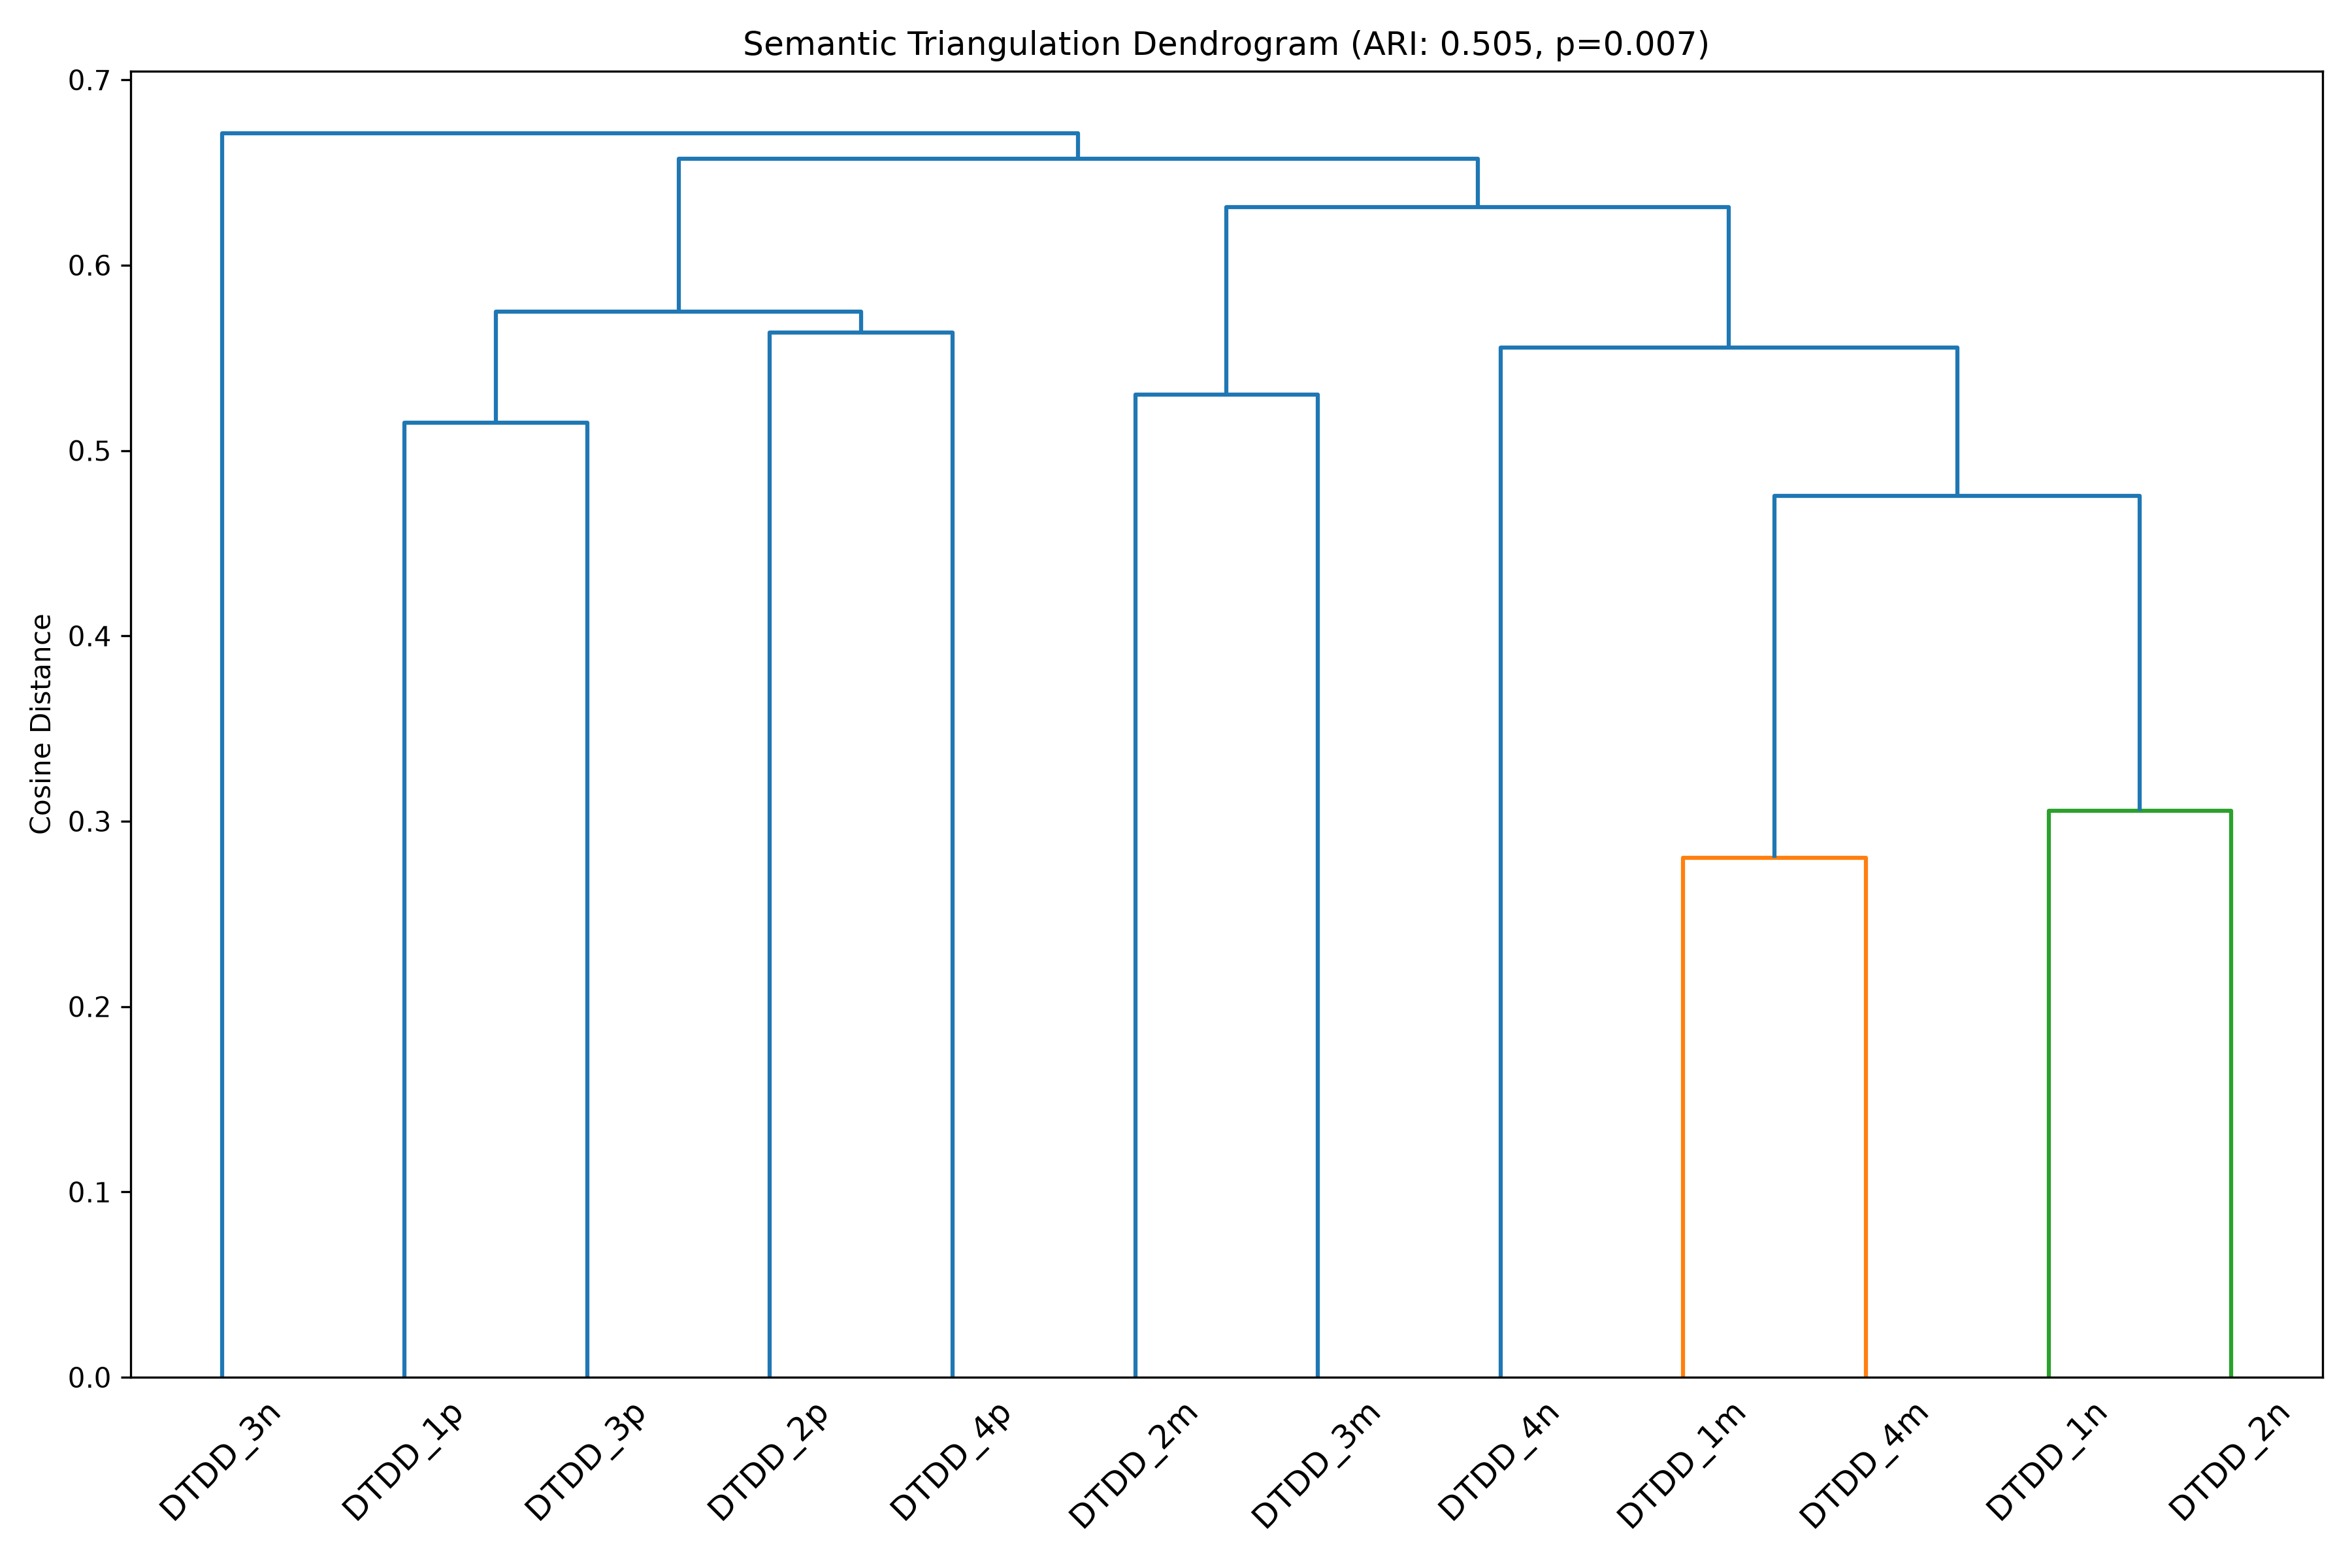
\includegraphics[width=\linewidth]{results/figures/layer4_semantic_dendrogram.png}
\caption{Hierarchical clustering dendrogram of DTDD item-text embeddings. Narcissism items partially fracture into the Machiavellianism branch.}
\label{fig:dendro}
\end{figure}

\subsection{Layer 5: Feature Importance and Robustness Testing}

The observed SHAP Divergence Index (SDI) was .2591, against a 500-iteration pseudo-trait null mean of .0953 ($SD = .0588$, $p = .0100$), exceeding chance-level partitioning of the same item set. The Rashomon Set analysis across XGBoost, Random Forest, and Elastic-Net showed a maximum $R^2$ variance of $\Delta = .019$ across architectures, but inspection of the per-trait values (Table~\ref{tab:rashomon}) reveals that Elastic-Net matched or exceeded XGBoost on psychopathy (.237 vs.\ .218) and narcissism (.144 vs.\ .132), while XGBoost led on Machiavellianism (.147 vs.\ .145). This indicates that the predictor--trait relationships are predominantly linear: the contribution of the supervised layer is therefore interpretive (SHAP geometry) rather than predictive. GMM clustering of local SHAP vectors showed decreasing BIC with more components (e.g., narcissism: 4097.6 at one component to 3373.0 at five components, with a markedly more gradual decline after two components)---weak evidence for individual-level subtypes. Five-fold cross-validation replicated satisfactorily between community and representative samples (e.g., psychopathy: .312 community vs.\ .237 representative); the student sample could not be evaluated due to missing auxiliary variables, so replication claims are restricted to the community--representative comparison.

\begin{table}[ht]
\centering
\caption{Rashomon Set comparison of out-of-sample $R^2$ across three architectures (identical train/test split).}
\label{tab:rashomon}
\footnotesize
\begin{tabular}{lccc}
\toprule
Trait & XGBoost & Elastic-Net & Random Forest \\
\midrule
Machiavellianism & .147 & .145 & .134 \\
Psychopathy      & .218 & \textbf{.237} & .219 \\
Narcissism       & .132 & \textbf{.144} & .126 \\
\bottomrule
\end{tabular}
\end{table}

\subsection{Integrated Summary of Evidence}
\label{sec:integrated}

Table~\ref{tab:evidence} summarises the direction of evidence across the baseline psychometric analyses and the five computational layers. Two families of results are visible. When the DTDD items are analysed in isolation, distinctiveness dominates: the 12-item network yields three Louvain communities, XGBoost recovers trait-specific primary drivers, CKA falls below its permutation null, semantic clustering partially separates the traits, and the SHAP Divergence Index exceeds its pseudo-trait null. When the same items are embedded in the full 88-item personality space, convergence dominates: all twelve DTDD items collapse into a single community and the three latent factors correlate at $r = .36$--$.62$. The Discussion treats this isolation-versus-context pattern as the central empirical tension the paper must explain.

\begin{table*}[ht]
\centering
\caption{Direction of evidence across baseline analyses and the five computational layers.}
\label{tab:evidence}
\footnotesize
\begin{tabular}{p{3.2cm}p{5.2cm}p{4.0cm}}
\toprule
Evidence source & Metric & Direction \\
\midrule
CFA (three-factor) & CFI = .941, TLI = .923, RMSEA = .077 & Distinctiveness \\
Latent correlations & $r = .363$--$.623$ & Convergence (partial) \\
Network, 12-item DTDD & 3 Louvain communities & Distinctiveness \\
Network, 88-item full space & 1 DTDD community (Dark Core Collapse) & Convergence \\
OLS predictors & Shared (agreeableness) + trait-specific (empathy, age) & Partial divergence \\
XGBoost / SHAP & Distinct primary drivers & Distinctiveness \\
CKA & .054 vs.\ null .089, $p < .005$ & Distinctiveness \\
Semantic ARI & .505, $p = .007$ & Distinctiveness (narcissism fractured) \\
Counterfactual & Agreeableness shared by Mach/Narc; empathy by Psych & Partial convergence \\
SDI & .259 vs.\ null .095, $p = .010$ & Distinctiveness (internal) \\
Rashomon & $\Delta R^2 = .019$; linear competitive with XGBoost & Null for ML superiority \\
\bottomrule
\end{tabular}
\end{table*}

\section{Discussion}

\subsection{Central Finding: Distinctiveness Within a Shared Structure}

The five computational layers, together with baseline psychometrics, yield two seemingly contradictory but complementary findings. Every metric examining the three traits in isolation---the DTDD-only network, XGBoost predictor patterns, CKA representations, semantic embeddings, and the SDI---convergently showed distinguishable functional, predictive, and representational patterns. Every metric examining the traits within a broader nomological context---the full 88-item network and latent factor correlations---showed convergence into a shared higher-order structure. This mirrors the prediction of Dark Factor theory \citep{moshagen2018}: dark traits are surface, partly distinct manifestations of a shared fundamental disposition. The appropriate conclusion is neither ``three fully independent traits'' nor ``one unitary factor,'' but three statistically specified dimensions nested within a strong general Dark factor, with two of the three (Psychopathy and Narcissism) retaining substantive specific variance and the third (Machiavellianism) functioning as a near-pure indicator of the general factor---consistent with \citet{vize2018} and with the bifactor results reported in Section~\ref{sec:baseline}.

\subsection{Machiavellianism and Psychopathy: A Distinction Without a Difference?}

Machiavellianism repeatedly occupied an intermediate, bridging position: its highest latent correlation was with psychopathy ($r = .623$), and its counterfactual sensitivity to agreeableness was shared with narcissism---consistent with \citet{miller2017}. However, psychopathy's distinctive predictor (empathy, not agreeableness) across Layers~2--3, and its complete semantic separation in Layer~4, indicate that psychopathy retains a distinct functional/predictive identity despite high latent overlap with Machiavellianism, suggesting the overlap may be more a shared-latent-variance phenomenon than a predictive/semantic one.

\subsection{The Narcissism Fracture and the Centrality of Agreeableness}

The overlap between narcissism and Machiavellianism was independently replicated at both the semantic clustering level (Layer~4) and the counterfactual level (Layer~3), converging on agreeableness. This aligns with \citet{vize2020}, who identified low agreeableness as a leading candidate for the Dark Triad's shared core, contrasted with callousness/low empathy \citep{paulhus2014}, here specifically tied to psychopathy. This supports a possible two-branch structure: an ``instrumental disagreeableness'' pole (Machiavellianism, narcissism) and an ``affective callousness'' pole (psychopathy)---an interpretation requiring confirmatory testing. Importantly, the latent CFA does not support the Narcissism Fracture as a covariance-structure phenomenon: the 2-factor model merging Machiavellianism with Narcissism ($\chi^2 = 6278.64$, $df = 53$, CFI = .793, TLI = .743, RMSEA = .141) fits substantially worse than the free three-factor model ($\chi^2 = 1838.65$, $df = 51$, CFI = .941, RMSEA = .077). In fact, it fits worse than the 2-factor model merging Machiavellianism with Psychopathy (CFI = .849, RMSEA = .120), despite the two trait pairs having nearly identical latent correlations ($r = .606$ vs.\ $.623$). The Narcissism Fracture is therefore a semantic (Layer~4) and feature-importance (Layer~3) phenomenon, not a latent-correlation one---and this three-level dissociation (latent fit, semantic organization, predictive feature importance) is itself a substantive finding, precisely the kind of dissociation that a single-level CFA or a single-level network cannot reveal.

\subsection{Position Within the Existing Literature}

Using tools entirely independent of CFA, this study converges with the Dark Factor framework \citep{moshagen2018}---itself derived from factor-analytic methods in large populations---that dark traits share an underlying disposition. This methodological convergence across unrelated analytic families constitutes a form of convergent validity for the Dark Core hypothesis. Explainable-AI tools (SHAP, CKA) additionally reveal higher-order interactions, nonlinear functional forms, and representational geometry not accessible to linear regression or CFA alone. The Rashomon analysis, however, qualifies the claim that nonlinearity is empirically necessary: linear models performed comparably, and the value of the explainable-ML layer lies primarily in interpretability of predictor structure rather than in superior predictive power.

\subsection{Limitations}
\label{sec:limitations}

\begin{enumerate}[leftmargin=1.2em,itemsep=0pt,topsep=2pt]
\item \textit{Limited explanatory power of supervised models.} Out-of-sample $R^2$ (.13--.22) restricts inferences to nomological overlap rather than the full latent constructs.
\item \textit{Interdependence of the SDI criterion and null.} Both actual scores and pseudo-trait nulls derive from the same 12 items, so the SDI null is not fully independent of the measurement system and should not support causal/ontological claims.
\item \textit{Conceptual overlap between predictors and criteria.} Agreeableness and empathy conceptually overlap with the Dark Triad constructs themselves, so observed distinctiveness/overlap may partly reflect content overlap rather than an independent underlying structure.
\item \textit{Small semantic-analysis sample.} Layer~4 rests on only 12 item texts and a single embedding model; stability across models (e.g., MPNet, BGE, E5) remains untested.
\item \textit{Non-causal counterfactual analysis.} Layer~3 identifies predictive-model leverage only, not causal relationships.
\item \textit{Symbolic regression complexity/overfitting risk.} Discovered equations (especially for psychopathy) are complex and treated as supplementary, not primary, evidence.
\item \textit{Student-sample constraints.} Missing auxiliary variables excluded the student sample from predictive modeling and cross-sample replication; replication claims are limited to the community--representative comparison.
\item \textit{Lower psychopathy-subscale reliability.} Lower internal consistency/stability for psychopathy (student-sample $\omega = .638$) may partly explain its apparent distinctiveness via measurement error rather than construct differences.
\item \textit{Cross-layer predictor mismatch for age.} Age was included in the supervised layers but not in the baseline OLS; the narcissism--age association reported in Layers~2--3 is therefore not directly comparable to the OLS $\beta$s.
\item \textit{Exploratory, non-preregistered analysis.} Findings are hypothesis-generating and require confirmatory, preregistered replication.
\item \textit{CKA permutation null underspecified.} The permutation null used for the CKA analysis was constructed by re-running the network with permuted labels rather than by a fixed geometric reference; because the trunk is shared across the three task heads, the residual CKA between head activations depends on the exact layer at which representations are compared. The reported CKA value should therefore be read as a within-model contrast, not as an estimate of population representational divergence.
\item \textit{Counterfactual grid bounds and prediction-variance compression.} Two artifacts qualify the Layer~3 percentages. First, the grid search did not standardize perturbation bounds across traits, so a feature with a wider empirical range admits larger counterfactual moves. Second, and more consequentially, the flip rate scales inversely with model $R^2$: the trait with the lowest explained variance (Narcissism, $R^2 = .132$) shows the highest flip rate (61.8\%), because predictions are compressed toward the median and require smaller perturbations to cross. Comparative claims across traits are therefore not supported by these percentages; only within-trait interpretation of the primary tipping feature is warranted.
\item \textit{Unsigned SHAP magnitude.} The SHAP Divergence Index uses mean absolute SHAP values, which discards the sign of predictor effects. Two predictors of equal magnitude but opposite direction (e.g., Neuroticism $\beta = -.138$ for Psychopathy vs.\ $+.120$ for Narcissism in Table~\ref{tab:ols}) are treated as similar rather than opposite. A signed directional SHAP comparison was not performed and would strengthen future versions of the index.
\end{enumerate}

\subsection{Suggestions for Future Research}

Three directions are proposed: (1) preregistered, confirmatory re-testing of the Narcissism Fracture and agreeableness/empathy centrality in independent samples; (2) robustness testing of Layer~4 across multiple embedding models and, where feasible, the 15-item DTDD variant with additional impulsivity/antisocial items; and (3) integration of the DT$^3$ framework with longitudinal designs to test temporal and individual-level stability of convergence/divergence patterns.

\section{Conclusion}

By integrating classical psychometrics with five independent layers of computational evidence---network psychometrics, supervised machine learning, counterfactual analysis, semantic embeddings, and cross-architecture robustness testing---this study provides convergent support for a middle-ground conclusion: Machiavellianism, psychopathy, and narcissism are three dimensions nested within a strong general Dark factor (ECV = .576, $\omega_H$ = .734), with Psychopathy and Narcissism retaining substantive specific variance ($\omega_{HS} = .450$ and $.532$) and Machiavellianism functioning as a near-pure indicator of the general factor ($\omega_{HS} = .036$; mean signed specific loading $\approx .15$). This distinctiveness is evident in predictive drivers, neural representations, and (partially) semantic organization, alongside considerable overlap---particularly between Machiavellianism and narcissism around agreeableness. Given the limited explanatory power of the supervised models and the exploratory, non-preregistered nature of this analysis, the findings should be regarded as hypothesis-generating rather than confirmatory. Nonetheless, the convergence of several independent methods toward a single conclusion illustrates the value of integrative psychology--explainable-AI approaches for classic questions of personality structure.

\section*{CRediT authorship contribution statement}
S.K.: conceptualisation, methodology, formal analysis, writing -- original draft, writing -- review \& editing.
K.M.J.: software, data curation, formal analysis, visualisation, writing -- review \& editing.

\section*{Declaration of generative AI and AI-assisted technologies}
Generative AI (a large language model) was used solely to assist with the LaTeX typesetting and formatting of this manuscript. It was not used for data analysis, statistical modelling, interpretation of results, or generation of scientific content. The authors reviewed all AI-assisted output and take full responsibility for the content of the publication.

\section*{Author Contributions}
Sabihe Khorshidi: psychological conceptualization, interpretation of findings, manuscript writing. Kian Mansouri Jamshidi: design and implementation of the computational pipeline, data analysis, code reproducibility. Both authors contributed to final manuscript writing and approval.

\section*{Data and Code Availability Statement}
The de-identified dataset analysed here is publicly available from the original validation study \citep{zivna2025} and its OSF project repository \citep{zivna2023osf}; no new data were generated. Complete code for preprocessing, baseline analyses, and the five computational layers is available at: \url{https://github.com/sirkianmj/dark_triad_triangulation}.

\section*{Conflict of Interest}
The authors declare no conflict of interest related to this research.

\begin{thebibliography}{99}
\footnotesize

\bibitem[Blondel et al.(2008)]{blondel2008}
Blondel, V.~D., Guillaume, J.-L., Lambiotte, R., \& Lefebvre, E. (2008). Fast unfolding of communities in large networks. \textit{Journal of Statistical Mechanics: Theory and Experiment}, 2008(10), P10008.

\bibitem[Chen \& Guestrin(2016)]{chen2016}
Chen, T., \& Guestrin, C. (2016). XGBoost: A scalable tree boosting system. In \textit{Proceedings of the 22nd ACM SIGKDD International Conference on Knowledge Discovery and Data Mining} (pp. 785--794).

\bibitem[Epskamp \& Fried(2018)]{epskamp2018}
Epskamp, S., \& Fried, E.~I. (2018). A tutorial on regularized partial correlation networks. \textit{Psychological Methods}, 23(4), 617--634.

\bibitem[Fisher et al.(2019)]{fisher2019}
Fisher, A., Rudin, C., \& Dominici, F. (2019). All models are wrong, but many are useful: Learning a variable's importance by studying an entire class of prediction models simultaneously. \textit{Journal of Machine Learning Research}, 20(177), 1--81.

\bibitem[Jonason \& Webster(2010)]{jonason2010}
Jonason, P.~K., \& Webster, G.~D. (2010). The Dirty Dozen: A concise measure of the Dark Triad. \textit{Psychological Assessment}, 22(2), 420--432.

\bibitem[Jones \& Paulhus(2014)]{jones2014}
Jones, D.~N., \& Paulhus, D.~L. (2014). Introducing the Short Dark Triad (SD3): A brief measure of dark personality traits. \textit{Assessment}, 21(1), 28--41.

\bibitem[Knitter et al.(2025)]{knitter2025}
Knitter, L.~A., Hoffmann, J., Eid, M., \& Koch, T. (2025). Measuring the dark triad: A meta-analytical SEM study of two prominent short scales. \textit{Frontiers in Psychology}, 15, 1469970.

\bibitem[Kornblith et al.(2019)]{kornblith2019}
Kornblith, S., Norouzi, M., Lee, H., \& Hinton, G. (2019). Similarity of neural network representations revisited. In \textit{Proceedings of the 36th International Conference on Machine Learning} (pp. 3519--3529). PMLR.

\bibitem[Leberecht et al.(2026)]{leberecht2026}
Leberecht, M., Nedderhoff, A., Zitzmann, S., \& Hecht, M. (2026). Comparing machine learning methods for predicting dark triad personality traits using social media text data. \textit{Journal of Research in Personality}, 120, Article 104690.

\bibitem[Lundberg \& Lee(2017)]{lundberg2017}
Lundberg, S.~M., \& Lee, S.-I. (2017). A unified approach to interpreting model predictions. In \textit{Advances in Neural Information Processing Systems 30} (pp. 4765--4774).

\bibitem[Miller et al.(2017)]{miller2017}
Miller, J.~D., Hyatt, C.~S., Maples-Keller, J.~L., Carter, N.~T., \& Lynam, D.~R. (2017). Psychopathy and Machiavellianism: A distinction without a difference? \textit{Journal of Personality}, 85(4), 439--453.

\bibitem[Moshagen et al.(2018)]{moshagen2018}
Moshagen, M., Hilbig, B.~E., \& Zettler, I. (2018). The dark core of personality. \textit{Psychological Review}, 125(5), 656--688.

\bibitem[Muris et al.(2017)]{muris2017}
Muris, P., Merckelbach, H., Otgaar, H., \& Meijer, E. (2017). The malevolent side of human nature: A meta-analysis and critical review of the literature on the Dark Triad (narcissism, Machiavellianism, and psychopathy). \textit{Perspectives on Psychological Science}, 12(2), 183--204.

\bibitem[O'Boyle et al.(2015)]{oboyle2015}
O'Boyle, E.~H., Forsyth, D.~R., Banks, G.~C., Story, P.~A., \& White, C.~D. (2015). A meta-analytic test of redundancy and relative importance of the Dark Triad and five-factor model of personality. \textit{Journal of Personality}, 83(6), 644--664.

\bibitem[Papageorgiou et al.(2019)]{papageorgiou2019}
Papageorgiou, K.~A., Benini, E., Bilello, D., Gianniou, F.-M., Clough, P.~J., \& Costantini, G. (2019). Bridging the gap: A network approach to Dark Triad, Mental Toughness, the Big Five, and perceived stress. \textit{Journal of Personality}, 87(6), 1250--1263.

\bibitem[Paulhus(2014)]{paulhus2014}
Paulhus, D.~L. (2014). Toward a taxonomy of dark personalities. \textit{Current Directions in Psychological Science}, 23(6), 421--426.

\bibitem[Paulhus \& Williams(2002)]{paulhus2002}
Paulhus, D.~L., \& Williams, K.~M. (2002). The Dark Triad of personality: Narcissism, Machiavellianism, and psychopathy. \textit{Journal of Research in Personality}, 36(6), 556--563.

\bibitem[Reimers \& Gurevych(2019)]{reimers2019}
Reimers, N., \& Gurevych, I. (2019). Sentence-BERT: Sentence embeddings using Siamese BERT-networks. In \textit{Proceedings of the 2019 Conference on Empirical Methods in Natural Language Processing} (pp. 3982--3992).

\bibitem[Rodriguez et al.(2016)]{rodriguez2016}
Rodriguez, A., Reise, S.~P., \& Haviland, M.~G. (2016). Evaluating bifactor models: Calculating and interpreting statistical indices. \textit{Psychological Methods}, \textit{21}(2), 137--150. \url{https://doi.org/10.1037/met0000045}

\bibitem[Shukla \& Upadhyay(2025)]{shukla2025}
Shukla, M., \& Upadhyay, N. (2025). Cold hearts and dark minds: A systematic review and meta-analysis of empathy across dark triad personalities. \textit{Frontiers in Psychiatry}, 16, 1546917.

\bibitem[Vize et al.(2020)]{vize2020}
Vize, C.~E., Collison, K.~L., Miller, J.~D., \& Lynam, D.~R. (2020). The ``core'' of the dark triad: A test of competing hypotheses. \textit{Personality Disorders: Theory, Research, and Treatment}, 11(2), 91--99.

\bibitem[Vize et al.(2018)]{vize2018}
Vize, C.~E., Lynam, D.~R., Collison, K.~L., \& Miller, J.~D. (2018). Differences among Dark Triad components: A meta-analytic investigation. \textit{Personality Disorders: Theory, Research, and Treatment}, 9(2), 101--111.

\bibitem[Wachter et al.(2017)]{wachter2017}
Wachter, S., Mittelstadt, B., \& Russell, C. (2017). Counterfactual explanations without opening the black box: Automated decisions and the GDPR. \textit{Harvard Journal of Law \& Technology}, 31(2), 841--887.

\bibitem[Wehner et al.(2021)]{wehner2021}
Wehner, C., Ziegler, M., G\"odeke, W., \& L\"ammle, L. (2021). Further inflaming the discussion or cooling down feelings? A network analysis of the Dark Triad and the Five Factor Model of personality. \textit{Personality and Individual Differences}, 175, Article 110717.

\bibitem[\v{Z}ivn\'{a} et al.(2025)]{zivna2025}
\v{Z}ivn\'{a}, K., Novak, L., Zidkova, R., Helvich, J., Tavel, P., \& Malinakova, K. (2025). Impulsivity, psychopathy, and the dark triad: A Czech validation of the Dirty Dozen scale. \textit{BMC Psychology}, \textit{13}(1), 1170. \url{https://doi.org/10.1186/s40359-025-03371-y}

\bibitem[\v{Z}ivn\'{a}(2023)]{zivna2023osf}
\v{Z}ivn\'{a}, K. (2023). \textit{Dark personality traits and their structure} [Data set]. OSF. \url{https://osf.io/8dp72}

\end{thebibliography}

\end{document}